\documentclass[a4paper]{article}

\usepackage[english]{babel}
\usepackage{verbatim}
\usepackage{graphicx}
\usepackage{listings}
\usepackage{color}
\usepackage{url}
\usepackage{enumitem, hyperref}

\title{Ein Versuch Algorithmen und Datenstrukturen in der Lehre der angewandten Computerwissenschaften grafisch zu simulieren}
\author{Armin Langhofer}
\date{\today}
\makeatletter

\usepackage[ngerman]{datetime}
\newdateformat{mygermandateformat}{\THEDAY{ten }\monthnamengerman[\THEMONTH] \THEYEAR}
\newdateformat{mygermanmonthformat}{\monthnamengerman[\THEMONTH] \THEYEAR}

\begin{document}
\iffalse
\maketitle 
\fi

\begin{titlepage}
	\centering
	
	
	{\huge \@title \par}
	
	\vspace{1.5cm}
	
	{\Large Masterarbeit \par}

	{\Large Zur Erlangung des Mastergrades \par}
	\vspace{1.5cm}
	
	{\Large an der Naturwissenschaftlichen Fakult\"at der Paris-Lodron-Universit\"at Salzburg \par}
	\vspace{11cm}

	Gutachter: Ao.Univ.Prof. Mag.Dr. Helge \textsc{Hagenauer}\par
	Fachbereich: Computerwissenschaften\par
	Eingereicht von \@author\space im \mygermanmonthformat\@date\par
	\vspace{2cm}


	\vfill
\end{titlepage}


\newpage

\tableofcontents

\newpage

\section{Einleitung}

\section{Anforderungen}
Ein System soll erarbeitet werden bei dem man einen Algorithmus grafisch veranschaulichen kann. Dabei soll man den Ablauf
\begin{enumerate}
\item steuern und
\item visualisieren
\end{enumerate}
k\"onnen.

\subsection{Steuerung}
Es soll m�glich sein, den Algorithmus im Einzelschnitt abarbeiten zu lassen. Folgende Funktionen sind denkbar:
\begin{enumerate}
\item Einzelschritt (vor)
\item Zur\"uck
\end{enumerate}

\subsection{Visualisierung}
Es soll m�glich sein, den Algorithmus im jeweiligen Zustand (grafisch) anzuzeigen. Die Visualisierung ist vom Algorithmus abh\"angig, denkbar sind:
\begin{enumerate}
\item B\"aume
\item Listen
\end{enumerate}

\section{Existierende Systeme}

Folgende bereits existierenden Systeme\cite{uavicse} werden untersucht:
\begin{enumerate}
\item \label{jawaa2} JAWAA \cite{jawaa2}
\item \label{trakla} TRAKLA2 \cite{trakala2}
\item \label{animal} ANIMAL \cite{animal}

\end{enumerate}

\subsection{Jawaa}

Leider war es nicht m"oglich w"aehrend des Zeitraumes der Entstehung dieser Arbeit online auf die Beispiele dieses Projektes zuzugreifen. Weder das Hinzuf�gen der gew"uenschten URLs in die Java-Sicherheitsausnahen noch ein lokaler Start ermg"oeglichte den Start der Beispiele. Auch nicht die Verwendung von diversen Browsern (IE, FF, Safai, Chrome) schuf Abhilfe.

\begin{figure}
	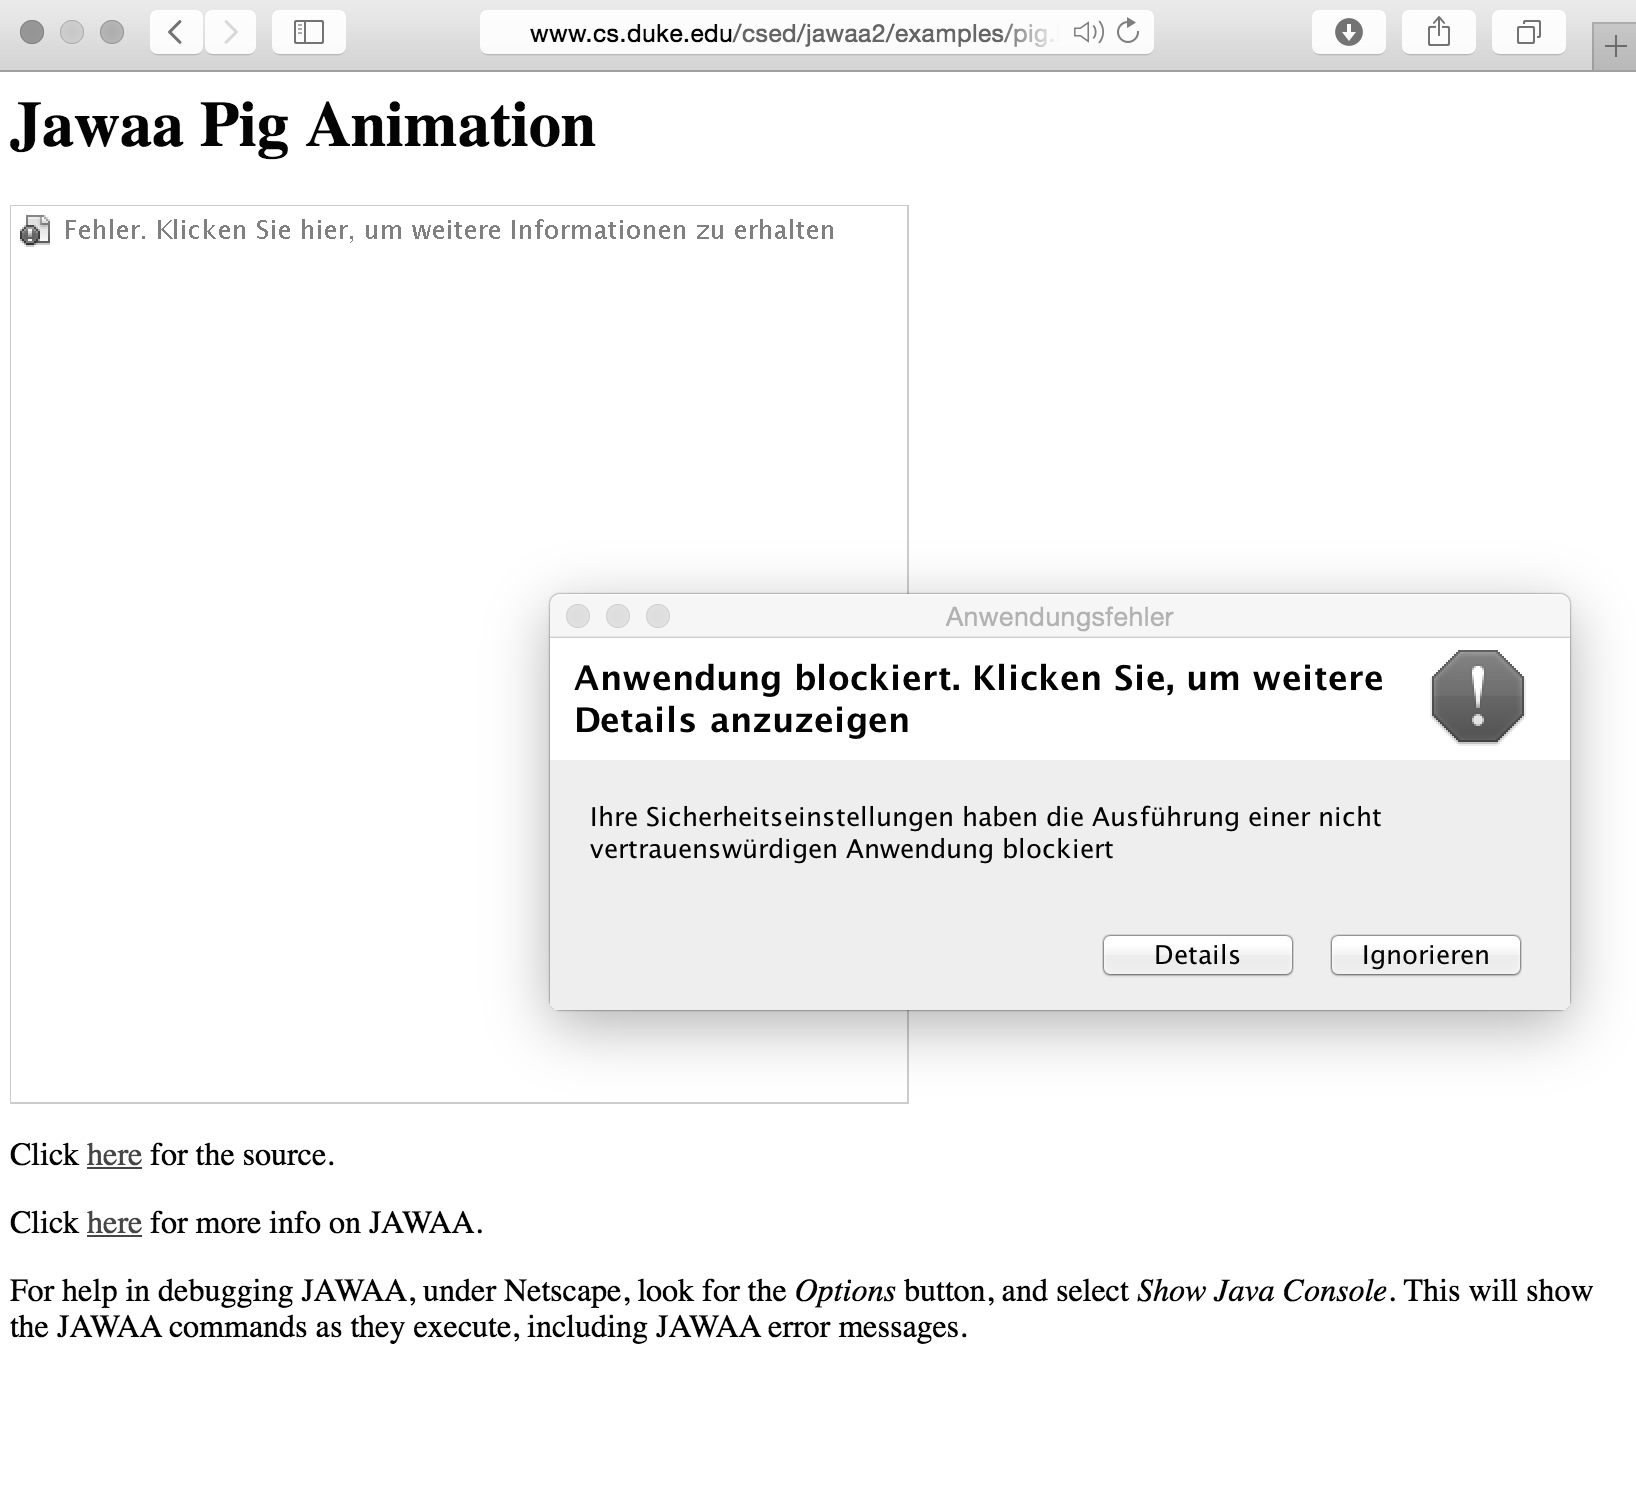
\includegraphics[scale=0.5]{img/jawaa.png}
	\caption[Jawaa's Java Applet not launching on current systems] {Jawaa's Java Applet not launching on current systems}
\end{figure}


\subsection{Trakala2}




\subsection{Animal}
Dieses Projekt war im Zeitraum der Entstehung dieser Arbeit nicht (mehr) verf\"ugbar.

\begin{figure}
	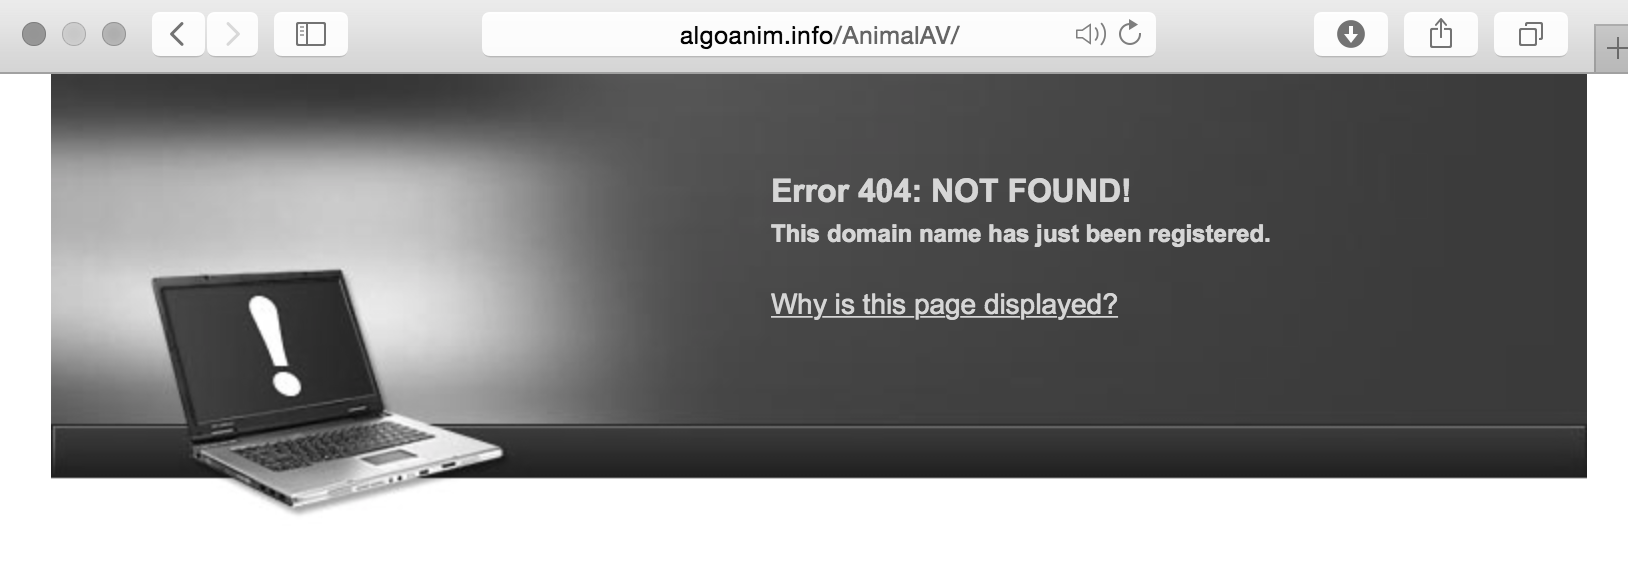
\includegraphics[scale=0.5]{img/animalav.png}
	\caption[Animal's Website not found] {Animal's Website not found}
\end{figure}


\newpage
\listoffigures

\newpage
\bibliographystyle{plain}
\bibliography{refs}

\end{document}
